\section{TAS (Test and Set)}

\textbf{TAS} è un'istruzione che:
\begin{itemize}
    \item \textbf{Controlla} se il bit più significativo dell'operando è 0 (semaforo libero);
    \item \textbf{Set} del bit più significativo a 1 (semaforo occupato) nel caso lo trovi libero. 
\end{itemize}

A seguito dell'operazione i bit N e Z dello SR vengono aggiornati. Questa operazione è atomica (indivisibile), quindi usa un solo ciclo read-modify-write. La sua principale applicazione è nei sistemi multiprocessore: infatti un processore che esegue TAS non può essere interrotto tra la fase di Test e la fase di Set, rendendo consistente l'operazione di acquisizione del semaforo. 
Il metodo di indirizzamento è indiretto o tramite registro. 

\subsection{Esercizio 1} \label{par:esercizio_2_1}
Due nodi B e C inviano K messaggi da N caratteri al nodo A, ognuno tramite una periferica PIA. Senza particolari ipotesi semplificative sulla priorità di un nodo rispetto ad un altro, scrivere il codice assembler eseguito dal nodo A in modo che:

\begin{itemize}
    \item Se il nodo B trasmette un messaggio ad A, A deve terminare la ricezione dell'intero messaggio prima di ricevere un eventuale messaggio da C.
    \item Analogamente, se il nodo C trasmette un messaggio ad A, A deve terminare la ricezione dell'intero messaggio prima di ricevere un eventuale messaggio da B. 
\end{itemize}

Il collegamento tra i dispositivi avviene tramite PIA secondo il meccanismo indicato precedentemente. Per la configurazione fare riferimento alla figura \ref{img:TAS_1}

\begin{figure} [!ht]
    \centering
    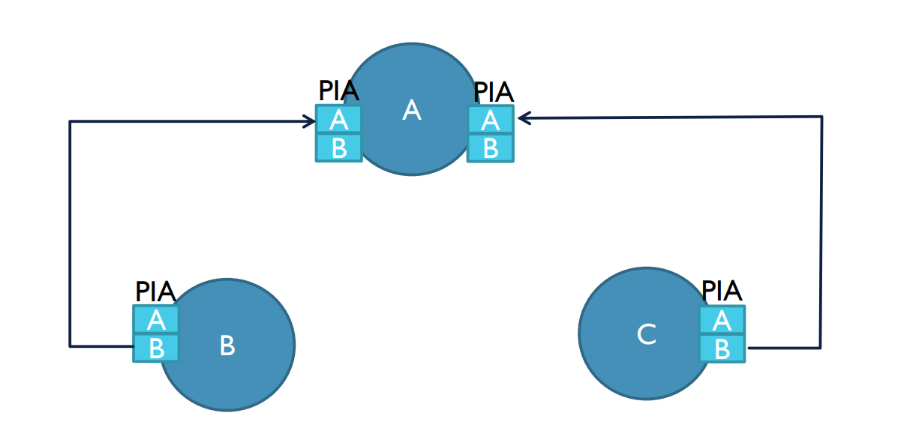
\includegraphics[width=0.5\textwidth]{img/TAS_1.png}
    \caption{Schema logico}\label{img:TAS_1}
\end{figure}

Possiamo considerare il nodo A come una risorsa condivisa dai nodi B e C. Siamo nel caso in cui è possibile utilizzare l'istruzione TAS: Prima di effettuare l'invio del messaggio, B e C devono verificare che A non sia impegnato con l'altro nodo. Questo è possibile farlo se A definisce una variabile \textit{possesso}, dove il valore 0 indica il possesso di B, 1 indica il possesso di C, -1 indica risorsa libera. L'accesso alla variabile \textit{possesso} deve essere mutualmente esclusivo, per evitare race conditions. Per questo motivo la variabile è acceduta tramit un lock, controllato e settato tramite TAS. 
Poichè stiamo utilizzando la PIA in configurazione tale per cui la ricezione di un messaggio dal nodo A causa interruzione, possiamo programmare l'ISR di A relativa alla ricezione di un messaggio da parte di B o da parte di C. 

\begin{itemize}
    \item \textbf{ISRB}: Per prima cosa si controlla che A non sia impegnato nella comunicazione con C, controllando la variabile possesso (in mutua esclusione). Se il possesso è di B (0) o è libero (-1) allora si può procedere all'invio, altrimenti B aspetta. 
    \item \textbf{ISRC}: Per prima cosa si controlla che A non sia impegnato nella comunicazione con B, controllando la variabile possesso (in mutua esclusione). Se il possesso è di C (1) o è libero (-1) allora si può procedere all'invio, altrimenti C aspetta.
\end{itemize}

Questo meccanismo è pericoloso in quanto permette il DeadLock. Serve un meccanismo per riprendere la ricezione sospesa. Il motivo per cui una ricezione possa essere sospesa è un'interruzione di priorità maggiore o un malfunzionamento della periferica. 

vediamo lo pseudocodice relativo alla ISRB:

\begin{lstlisting}[language=C]
    if (sem == verde){      \\istruzione atomica TAS
        sem = rosso;
        if (possesso != 1){ \\possesso non di C
            possesso = 0;
            sem = verde;
            leggo_car_b();
            car_counter_b++;
            if (car_counter_b==N){ \\fine trasmissione
                if(c_sospeso){
                    possesso = 1; \\possesso di C
                    leggo_car_c();
                    car_counter_c++;
                }
                else{
                    possesso=-1;
                }
            }
        }
        else{
            sem = verde;
            leggo_car_c();
            car_counter_c++;
        }
        return 0;
    }
    return 0;
\end{lstlisting}

Nel codice vediamo che tramite l'istruzione TAS controlliamo se il semaforo è verde e lo settiamo subito a rosso. Quindi, se il possesso non è di C, B prende il possesso e reimposta il semaforo a verde, dopodichè procede con la lettura del prossimo carattere. Se il messaggio è finito, se C è sospeso C viene sbloccato attraverso la lettura del carattere di C, altrimenti viene liberato il possesso. Se il possesso è già di C, C potrebbe aver provato ad accedere alla sezione critica (invio del messaggio) mentre B controllava in mutua esclusione il possesso. In questo caso, C viene sbloccato attraverso la lettura di un carattere. Se in primo luogo B trova il semaforo rosso, B viene sospeso.
Per verificare se B o C sono sospesi, si controlla nel registro di stato se CRA7B o CRA7C sono alti (interruzione pendente). 
Lo pseudocodice della ISRC è praticamente speculare a quello presentato sopra. Presentiamo di seguito l'implementazione commentata dell'esercizio.

\subsubsection{Nodo A}
\begin{lstlisting}
            ORG     $8000
MSG_CHAR    EQU     3
N_ITER      EQU     5
N_MEX_B     EQU     2   * Msg per iterazione
N_MEX_C     EQU     3   * Msg per iterazione 

***PIA***
PIADA       EQU     $2004
PIACA       EQU     $2005
PIADA2      EQU     $2008
PIACA2      EQU     $2009

***VARIABILI DEL SISTEMA A***
BUFF_B      DS.W    64
BUFF_C      DS.W    32
CTR_CH_B    DC.W    0
TOT_B       DC.W    0
CTR_MS_B    DC.W    0
CTR_CH_C    DC.W    0
TOT_C       DC.W    0
CTR_MS_C    DC.W    0

END_B       DC.W    0
END_C       DC.W    0
K           DC.W    0

            ORG     $8200
INIT        JSR     INIT
            MOVE.W  SR,D1 
            ANDI.W  #$D8FF,D1 
            MOVE.W  D1,SR 
LOOP        JMP     LOOP

INIT        MOVE    #$0,PIACA 
            MOVE    #$0,PIADA 
            MOVE    #%00100101,PIACA 
            MOVE    #$0,PIACA2
            MOVE    #$0,PIADA2 
            MOVE    #%00100101,PIACA2 
            RTS

IB          CMP.W   #1,END_B
            BEQ     IB_RTE 
            MOVEM.L D0-D2/A0,-(SP)
            MOVE.W  TOT_B,D0
            MOVE.W  CTR_CH_B,D1 
            MOVEA.L #BUFF_B,A0 
            MOVE    PIADA,(A0,D0)
            ADDI.W  #1,D0 
            MOVE.W  D0,TOT_B
            ADDI.W  #1,D1 
            MOVE.W  D1,CTR_CH_B 
            CMP.W   #MSG_CHAR,D1
            BNE     EIB
            MOVE.W  #0,CTR_CH_B
			MOVE.W	CTR_MEX_B,D1
			ADDI.W 	#1,D1
			MOVE.W 	D1,CTR_MEX_B
			CMP.W  	#N_MEX_B_ITER,D1
			BNE		EIB
			MOVE.W 	#1,END_B
			CMP.W	#1,END_C
			BNE 	EIB 			
			MOVE.W 	K,D2
			ADDI.W	#1,D2
			MOVE.W	D2,K
			CMP.W	#N_ITER,D2
			BEQ		EIB			
			MOVE.W	#0,END_B
			MOVE.W	#0,END_C
			MOVE.W	#0,CTR_MEX_B
			* Recupera il messaggio di C se si era bloccato.
			MOVE.B  PIACA2,D0 	
			ANDI.B  #$80,D0
			BEQ		EIB
			* Aggiorna i contatori e poi leggi il caratteri
			MOVE.W 	TOT_C,D0
			MOVE.W	D0,D1
			ADDI.W	#1,D1
			MOVE.W	D1,TOT_C
			MOVE.W #1,CTR_CH_C
			MOVEA.L 	#BUFF_C,A0
			MOVE.B	PIADA2,(A0,D0)
EIB			MOVEM.L (SP)+,D0-D2/A0
IB_RTE		RTE 

IC     		CMP.W   #1,END_C
			BEQ     IC_RTE
			MOVEM.L D0-D2/A0,-(SP)
			MOVE.W  TOT_C,D0
			MOVE.W  CTR_CH_C,D1
			MOVEA.L #BUFF_C,A0
			MOVE.B  PIADA2,(A0,D0)
			ADDI.W  #1,D0
			MOVE.W  D0,TOT_C	
			ADDI.W  #1,D1       
			MOVE.W 	D1,CTR_CH_C	
			CMP.W 	#MEX_CHAR,D1
			BNE 	EIC
			MOVE.W 	#1,END_C
			CMP.W	#1,END_B
			BNE 	EIC
			MOVE.W 	K,D2
			ADDI.W	#1,D2
			MOVE.W	D2,K
			CMP.W	#N_ITER,D2
			BEQ		EIC
			MOVE.W	#0,END_B
			MOVE.W	#0,END_C
			MOVE.W	#0,CTR_MEX_B
			* Recupera il messaggio di C se si era bloccato.
			MOVE.B  PIACA,D0 	
			ANDI.B  #$80,D0
			BEQ		EIC
			* Aggiorna i contatori e poi leggi il caratteri
			MOVE.W 	TOT_B,D0
			MOVE.W	D0,D1
			ADDI.W	#1,D1
			MOVE.W	D1,TOT_B
			MOVE.W 	#1,CTR_CH_B
			MOVEA.L BUFF_B,A0
			MOVE.B	PIADA2,(A0,D0) 
EIC			MOVEM.L (SP)+,D0-D2/A0
IC_RTE		RTE 
\end{lstlisting}

Vediamo il codice inerente al sistema B:

\begin{lstlisting}
            ORG     $8000
DIM         EQU     3
MES         DC.B    1,2,3,0
CNT         DC.W    0
PIADB	    EQU	    $2006
PIACB	    EQU	    $2007

ORG	$8200
INIT	    JSR	    INIZIALIZZA
	
*Invio dimensione
            MOVE.W 	#DIM,D3	
            MOVEA.L	#PIADB,A0
            MOVEA.L #MES,A1
            MOVE.W 	#1,CNT * Inizia scrivendo 1 nel contatore di bytes		
            MOVE.W	CNT,D0	* D0 mantiene sempre il conteggio di bytes
            
            MOVE.W	SR,D1
            ANDI.W	#$D8FF,D1	*maschera per le interruzioni. 
            MOVE.W	D1,SR
            MOVE.B	(A0),D2		* Effettua la lettura fittizia
            MOVE.B 	(A1),(A0)	* Scrivi il primo messaggio

LOOP	JMP	LOOP


INIZIALIZZA	
            MOVE.B	#0,PIACB
            MOVE.B	#$FF,PIADB
            MOVE.B	#%00100101,PIACB
            RTS

*interruzione livello 4 mappato a $70
	        ORG	$8800
INT4        MOVE.B 	(A0),D2 * Lettura fittizia
	        MOVE.B 	(A1,D0),(A0) * Invia il carattere successivo
	        ADDI.W 	#1,D0
	        CMP.W	D3,D0
	        BNE		EI4
	        MOVE.W	#0,D0
EI4 	    RTE
END	        INIT

\end{lstlisting}

Il sistema C è praticamente speculare.

\subsection{Esercizio 2 - Prova intercorso 2023}
Un sistema è compoto da 3 unità (A,B,C) tra loro collegate mediante due periferiche parallele che interconnettono A con B e A con C rispettivamente. Il sistema opera effettuando k iterazioni (k>2), in ciascuna delle quali A deve ricevere globalmente 2 messaggi di N caratteri da B e 1 messaggio di N caratteri da C (N>2). I messaggi da B e da C possono essere ricebuti in un ordine qualsiasi ma non deve essere mai possibile ricevere caratteri appartenenti a messaggi diversi intervallati tra di loro.
Vediamo lo pseudocodice relativo alla ISRB:

\begin{lstlisting}[language=C]
    if (sem == verde){      \\istruzione atomica TAS
        sem = rosso;
        if (possesso != 1 && end_B == 0){ 
            possesso = 0;
            sem = verde;
            leggo_car_b();
            car_counter_b++;
            if(car_counter_b == N){
                mex_counter_b++;
                if(mex_counter_b == N_mex_b){
                    end_B = 1;
                }
                if(c_sospeso){
                    possesso = 1; \\possesso di C
                    leggo_car_c();
                    car_counter_c++;
                }
                else{
                    possesso=-1;
                }
            }
        }
        else{
            sem = verde;
            leggo_car_c();
            car_counter_c++;
        }
        return 0;
    }
    return 0;
\end{lstlisting}

La differenza rispetto all'esercizio \ref{par:esercizio_2_1}, B in questo caso per procedere deve controllare sia che la variabile possesso non sia di B, sia che A non abbia già ricevuto il numero di messaggi per quell'iterazione. Dopo la ricezione del carattere, non solo viene gestito il contatore relativo ai caratteri nel messaggio, ma anche un contatore che tiene conto del numero di messaggi ricevuti nella corrente iterazione. Se questo numero diventa uguale a N, si pone $end_B = 1$, e alla successiva interruzione non si riceverà alcun carattere, ma si sveglierà C se necessario e si uscirà. 
